\chapter{Weiterentwicklung eines Clients zu einem Messeprototyp}
\label{cha:weiterentwicklung-messeprototyp}
Nach der Entscheidung für die Weiterentwicklung der nativen Android-App, begann die Planung der möglichen Erweiterungen. Dabei wurden besonders Performance- und Stabilitätsaspekte in den Vordergrund gestellt. Darüber hinaus sollte aber auch die Oberfläche einem Messeprototyp entsprechend verbessert werden und Funktionen, die aus den Kann-Kriterien des Pflichtenheftes entspringen, umgesetzt werden, um einen größeren Funktionsumfang präsentieren zu können.

\section{Anpassungen der Ablauflogik}
\label{sec:anpassungen-ablauflogik}
Die Ablauflogik der nativen App wurde weitestgehend beibehalten, da die Planung im Vorfeld schon eine komplette \textit{User-Story} vorgesehen hat. So muss man sich zuerst anmelden, um dann durch die Trainingspläne und Übungen navigieren zu können und abschließend die Möglichkeit hat ein Training einzutragen. Demnach sind in diesem Sinne keine Verbesserungen oder Änderungen nötig.\\
Da die Anzeigelogik keiner großen Anpassung bedarf, wurde sich darauf konzentriert, Aspekte der  Stabilität und der Leistungsfähigkeit der App zu verbessern haben. So wurde die Synchronisation aus den Methoden der GET- und POST-Abfragen extrahiert und zentralisiert (siehe Kapitel \ref{ssec:cache-unsere-funktionsweise}).\\
Die Funktionalität des Caches wurde nur hinsichtlich der Synchronisation mit dem Server angepasst. Darüber hinaus wurden keine Änderungen vorgenommen. Das Synchronisieren erfolgt jeweils beim Abrufen von Daten vom -, sowie beim Übertragen von Daten zum Server.\\
Die Abbildung \ref{pic:nat-RecentOnline} verdeutlicht den neuen Ablauf der Synchronisation. \\
%Sequenzdiagramm-RecentOnline
\begin{figure}[!h]
\centering
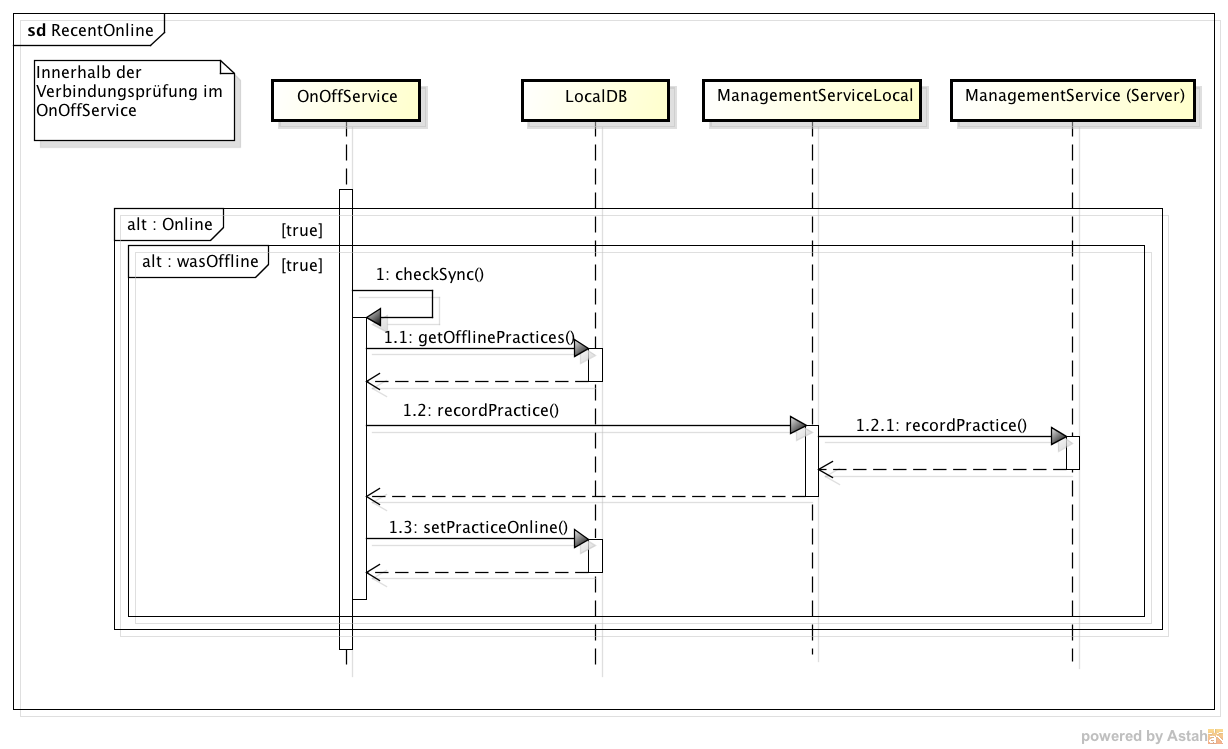
\includegraphics[width=\linewidth]{content/images/fITNat-RecentOnline}
\caption{Squenzdiagramm \textit{RecentOnline}}
\label{pic:nat-RecentOnline}
\end{figure}

Bedingung zum Start des Synchronisationsvorgangs ist, dass die Applikation aktuell eine Verbindung zum Server besitzt und im vorhergehenden Status noch offline war. Falls dann im Vorfeld Daten angelegt wurden, die nur lokal gespeichert werden konnten, werden diese ausgelesen, auf dem Server gespeichert und in der lokalen Datenbank wieder als synchronisiert gekennzeichnet.\\
In zweiten Meilenstein wurde der Programmcode überarbeitet, um die Umsetzung der weiteren Funktionen, welche das Pflichtenheft für diese Meilenstein vorsieht, zu erleichtern. \\
Im Folgenden ist es nunmehr nötig die Daten, die während der Zeit im Offline-Modus angelegt wurden, in der Methode \textit{checkSync()} einzutragen. Unter der vorherigen Architektur hätte die Logik in jede Verbindnungsoperation kopiert werden müssen. Dies hätte zu einer hohen Anzahl an Redundanzen im Code geführt. Diese Redundanz sollte unbedingt umgangen werden. Deshalb ist diese zentralisierte Stelle zum Überprüfen der zu übertragenden Daten umgesetzt worden.
\section{Anpassungen der Oberfläche}
\label{sec:anpassungen-oberflaeche}
Die Oberflächen wurde dahingehend angepasst, dass ein durchgängige Design über die ganze \gls{UserStory} hinweg, erkennbar ist. Diese kann vollständig im Anhang eingesehen werden (siehe \ref{sec:UserStory}).\\ 
Die Oberfläche, insbesondere Schaltflächen und Dialoge wurden in diesem Schritt angepasst.\footcite{Android-Oberflaechen} Dabei wurden zwei Designs umgesetzt: eine für den Login- und eine für den Registrieren-Button. Dazu war es nötig eine \ac{XML}-Datei anzulegen, welche die Eigenschaften der Schaltfläche beschreibt (siehe Quellcode-Beispiel \ref{lst:BtnSignInNotClicked}):
\lstinputlisting[caption=Design des Login-\textit{Buttons}, label=lst:BtnSignInNotClicked, style=xml]{content/listings/ButtonSignInStyle.xml}

Weiterhin wurden die Dialogfenster mit Animationen versehen, um eine zum Betriebssystem passendes Verhalten zu erzeugen. Dazu musste, äquivalent zur Layout-Datei für die Schaltflächen, eine \ac{XML}-Datei angelegt werden, welche die Bewegungen des Fensters beschriebt (siehe Quellcode-Beispiel \ref{lst:slideRight}).
\lstinputlisting[caption=Dialog-Animation, label=lst:slideRight, style=xml]{content/listings/slide_right.xml}
Weiterhin wurden die Icons zur Anzeige des Verbindungsstatus ausgetauscht um diese an das neue Design anzupassen. Als letztes wurde ein App-Icon hinzugefügt, welches auf dem Home-Screen des Endgerätes angezeigt wird. 

\section{Implementierung der Statistik}
\label{sec:implementierung-statistik}
Um Fortschritte des Nutzers anzeigen zu können, wurde eine Übersicht mit den eingetragenen Trainingsleistungen implementiert. Diese ist für jede Übung über einen längeren Klick auf das Übungs-Feld erreichbar. In dem Balkendiagramm ist das Produkt aus dem Trainingsgewicht, der Wiederholungszahl und der Satzzahl dargestellt. Ein Screenshot der Oberfläche liegt dem Anhang bei (siehe \ref{pic:natAppStatistik})\\
Zur Darstellung wurde die \textit{Xamarin-Extension BarChart} verwendet. Das Paket  wurde in das Projekt eingebunden und kann durch einen einfachen Aufruf mit der Übergabe eines Daten-\textit{Arrays} verwendet werden (Quellcode: \ref{lst:statistik}).\\
Zur Generierung der Diagramm-Daten waren Informationen über die Übung, den Trainingsplan und den \textit{User} nötig. Diese Daten werden über einen Intent an die \textit{StatisticActivity} übergeben, in welcher dann die benötigten Daten abgerufen werden.
\lstinputlisting[caption=Statistik \textit{Activity}, label=lst:statistik, style=sharpc]{content/listings/StatisticActivity.cs}

\section{Fazit aus Meilenstein 2}
\label{sec:fazit-meilenstein-2}
Zusammenfassend kann festgehalten werden, dass der zweite Meilenstein zur Optimierung der nativen Android-Applikation beigetragen hat. Dies geschah sowohl in der Programmlogik als auch durch die Anpassungen der Oberflächen. \\
So konnte durch das Auslagern der Synchronisation Last vom dem \textit{UIThread} genommen werden. Die daraus folgenden Vorteile wurden bereits in Kapitel \ref{cha:native-app} vorgestellt.\\
Bei der Entwicklung eines Messeprototypen ist eine ansprechende Oberfläche von großer Bedeutung für die Akzeptanz durch den späteren Nutzer. Diese Anforderung wurde im ersten Meilenstein zurückgestellt, um einen Fokus auf den technischen Vergleich legen zu können. Nachdem nun im ersten Meilenstein eine für die Aufgabenstellung passende technische Grundlage entstanden ist, konnte sich in diesem Meilenstein auf die Optimierung des Aussehens fokussiert werden.\\
Die Statistik, ein Kann-Kriterium im Pflichtenheft (siehe Kapitel\ref{sec:Pflichtenheft}), wurde zusätzlich umgesetzt, um die Nutzerfreundlichkeit weiter zu steigern. Als Nebeneffekt wurden weitere Kenntnisse im Umgang mit langen Klicks und der \textit{BarChart-Extension} gesammelt.\\

Abschließend kann festgehalten werden, dass der zweite Meilenstein der nativen Applikation die letzten Verfeinerungen zum Prototypen gegeben hat.\\
Der Prototyp besitzt nun eine \gls{UserStory}, die alle benötigten Funktionen für die Entwicklung einer vollends ausgereiften \gls{App} beinhaltet. So kann die Funktionalität des Speicherns eines Trainings auf das Speichern von Übungen und Trainingsplänen übertragen werden. Zudem kann das Abrufen von weiteren Daten, zum Beispiel für die Umsetzung von Administrator-Funktionen, mit den bestehenden Möglichkeiten umgesetzt werden.

%UserStory
\begin{figure}[!htbp]
\centering
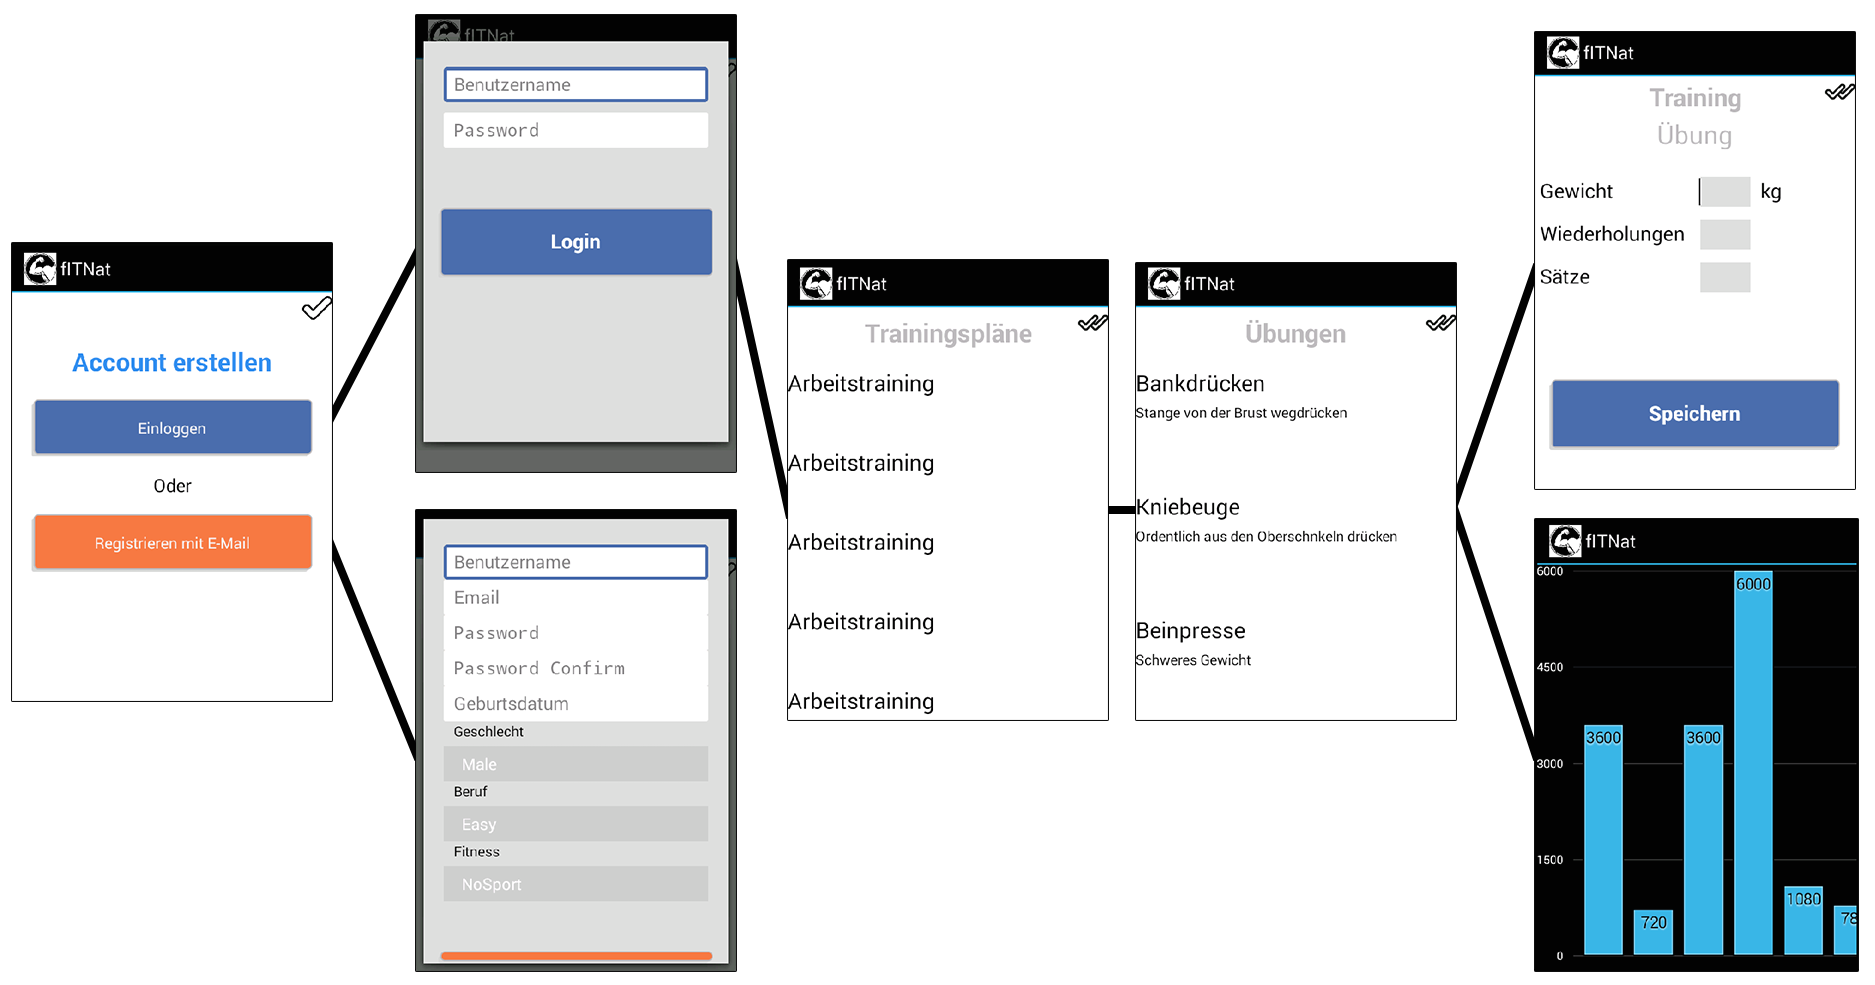
\includegraphics[width=\textwidth, angle={90}]{content/images/UserStory}
\caption{UserStory}
\label{pic:UserStory}
\end{figure}


In der Abbildung \ref{pic:UserStory} ist die Übersicht der Oberflächen zu erkennen. Größere Abbildungen sind im Anhang unter Abschnitt \ref{sec:UserStory} zu finden. Darüber hinaus sind auch die Verbindungen zwischen den Oberflächen eingezeichnet, um zeigen, wie der \textit{Workflow} verläuft.\\
Der Einstieg des Benutzers in die \gls{Android}-\gls{App} geschieht über die Startseite (siehe Abbildung \ref{pic:natAppStartseite}), die die Auswahl zwischen Login und Registrierung darstellt. Diese Oberfläche wird nur für Nutzer angezeigt, welche sich noch nicht an der \gls{App} angemeldet haben. \\
Wählt der Benutzer die Registrierung, gelangt er zum Registrieren-Dialog (siehe Abbildung \ref{pic:natAppRegistrierung}). Um diese Funktion nutzen zu können, muss das Gerät eine Verbindung zum Server besitzen. \\
Wählt der Nutzer, statt der Registrierungsschaltfläche, die Schaltfläche zum Anmelden, erscheint der Login-Dialog (siehe Abbildung \ref{pic:natAppLogin}). Um sich offline anmelden zu können, muss ein Nutzer sich einmal an der Applikation angemeldet haben, während diese eine Verbindung zum Web Service besessen hat. Dies ist nötig, da mit die \gls{App} validieren kann, ob die eingegebenen Daten serverseitig valide sind. Ist dies der Fall, werden sie lokal gespeichert, sodass sich ein Nutzer fortan auch lokal mit den gespeicherten Anmeldedaten autorisieren kann.\\
Nach einem erfolgreichen Anmeldung an der \gls{App}, sei es offline oder online, werden die Trainingspläne des Benutzers als Liste angezeigt (siehe Abbildung \ref{pic:natAppTrainingspläne}). Durch einen Klick auf den entsprechenden Plan, öffnet sich eine neue Seite mit den zu diesem Plan zugewiesenen Übungen (siehe Abbildung \ref{pic:natAppÜbungen}). Auf dieser werden die Übungen mit Namen und Beschreibung aufgelistet. Der Benutzer hat nun zwei Möglichkeiten, um zu interagieren: 
\begin{itemize}
\item Zum einen kann man durch das Auswählen einer Übung zu der Trainingsseite gelangen (siehe Abbildung \ref{pic:natAppTraining}). Auf dieser Seite kann der Benutzer dann die Daten für diese Übung zu einem Training eintragen. Benötigt werden dazu das Gewicht, die Anzahl der Sätze und die Wiederholungszahl.
\item Als zweite Möglichkeit kann durch einen langen Klick auf eine Übung eine Statistik zu den dazu eingetragenen Trainings aufgerufen werden. Diese Statistik wird als Balkendiagramm angezeigt und gibt einen Überblick über die Leistungen des Benutzers. Der Index berechnet sich als Produkt der eingetragenen Werte Gewicht, Satzzahl und Wiederholungen.
\end{itemize}
Werden neue Daten eingetragen, erscheinen diese, unabhängig von Verbindungsstatus sofort in der Statistik (siehe Abbildung \ref{pic:natAppStatistik}). Um in der Statistik alle Daten angezeigt zu bekommen, muss diese im Online-Modus aufgerufen werden, um die Daten auf das Gerät laden zu können. Wird die Statistik im Offline-Modus zum ersten Mal aufgerufen, werden nur die offline angelegten Trainings angezeigt.